\section{Methedology}
\subsection{General Setups}
Initially, we need to determine the data types to be used and define macros for 
assertions and helper functions to ensure that the program can detect common bugs 
and report their locations. 
These features can also be disabled in the release version for performance optimization. 
Such details are defined in the \texttt{assert.hpp}, \texttt{helper.hpp}, 
and other related header files located in the subfolder.

\subsection{Template Multi-dimension Matrix Detail Design}
The FDTD method is a type of FDM. 
The main idea behind FDM is briefly outlined in Section \ref{SEC:FDM}. 
The challenge lies in implementing it in a computer system to ensure it runs both correctly and efficiently.
Also, the data types I am using for storing sizes are unit32\_t and unit64\_t while I used them 
as Dworld and Qworld respectively, also are defined as size\_type and super\_size\_type in \_\_detail namespace.

\subsubsection{Performance Balancing}
\paragraph{Template Class}
Instead of doing this by using hierarchy in C++, which will cause the memory of object becomes complicated and unpredictable,
and leading to scattered data members between base and derived class objects.
This scattering can increase the cache misses which accessing these members, as the data might not be contiguous in memory.
Also, with deep inheritance hierarchies, program has higher change to occur diamond problems, since it increases the code complexity.
In detail, the diamond problem leads the duplicate inheritance and ambiguity in the method resolution, which will drop performance down again.
Although, it is solvable by using \texttt{virtual} inheritance, but again, it increase the complexity.

In such case, I chose to use template class to design the matrix object, which implement compile-time polymorphism as opposed runtime polymorphism
provided by inheritance and virtual functions. 
With such template design, the compiler makes the decisions about which function or class instantiate is made at compile time, eliminating 
the need for \texttt{vtable}s and indirect function calls, which leads to more efficient code. 

\paragraph{Memory Management}
Rather than using the standard library's (STL) vector module, 
which can be slower due to the overhead of row pointers, 
I opted to build the Matrix object using a unique pointer 
(
  \texttt{std::unique\_ptr}
), which includes only basic features such as reset, swap, and most importantly, 
a destructor that automatically deletes pointers. 
This approach enhances the safety of memory management in our programs.
Additionally, from a safety perspective, 
given that I implemented many features within the matrix object, 
I followed standard library conventions for naming. 
This includes using the \texttt{\_\_detail} namespace within namespace \texttt{multi\_array} to 
hide objects and features that are not intended for direct use by the end user.

\subsubsection{Template Object Design of Matrix Shape}

\paragraph{Strides} 
Besides that, in the multidimensional cases, the size in each dimension is not enough for accessing 
variables, this is where we need the \texttt{strides} member variable, which stores the 
number of element the operator needs to skip in each dimension.
The \texttt{\_\_multi\_array\_shape} object is encapsulated within 
the \texttt{\_\_detail} namespace and serves as a member variable of the later template object for the multi-dimensional matrix. 
This object includes a member variable defined using the STL vector, as the shape object primarily stores the sizes for each dimension, 
which typically requires only a small amount of space. 
Additionally, this object provides member functions to access the size of a given dimension. 
\begin{algorithm}
  \caption{Stride implementation}
  \begin{algorithmic}[1]
    \STATE \texttt{dims}    \hfill \# STL vector, stores the matrix's size in each dimension.
    \STATE \texttt{strides} \hfill \# STL vector, has the same size with dims.
    \STATE n = dims.size()  \hfill \# Store the dimension of matrix.
    \STATE strides[d-1] = 1; \hfill \# Stride is 1 in the first dimension.
    \FOR{ d = n - 1; d > 0; --d }     
      \STATE strides[d-1] = strides[d] * dims[d] \hfill \# Determine stride in the latter dimension.
    \ENDFOR
    \RETURN \texttt{strides}
  \end{algorithmic}
\end{algorithm}


\paragraph{Performace Balancing}
In certain scenarios, 
we only require the shape information of a matrix without needing to access the entire matrix object. 
Accessing the shape information through well-defined operators is a more efficient way to 
handle multidimensional matrices. 
This is particularly crucial in parallel programming, where understanding 
the shape of a matrix is of critical importance. 
Sometimes, a process may need to know the shape of matrices stored on other processes. 
In such cases, using this matrix object as a local variable within functions increases the 
likelihood that the compiler will store it in a register, 
which is generally faster than using heap or stack memory.
In addition, it includes check and cast functions that allow the user to verify if the template data type \texttt{\_\_T} is signed using \texttt{constexpr}. 
The \texttt{constexpr} keyword ensures that this check occurs at compile time, and if the data type is not legal, 
the program will assert and provide a message indicating that the indexing value must be a non-negative number. 


\subsubsection{Template of Multi-dimensional Matrix Implementation}
The Matrix in this project is designed to support various data types in C++. 
Consequently, the matrix is implemented as a template class with several essential features, template 
variable \texttt{\_\_T} and \texttt{\_\_NumD}, for the value data type and number of dimension, 
also including iterators, swap functionality, fill operations, and support for the IO stream operator \texttt{<<}. 
To facilitate this, the \texttt{\_\_array\_shape} object is used to explicitly manage and access the array's shape information. 


\paragraph{Operator \texttt{()}}
The hard part of this object designed is the support template number of dimension, whereas the dimension 
is integer not less than $1$,
the operator of access element is designed by following algorithm
\begin{algorithm}
  \caption{Operator \texttt{(Ext ... exts)} of template matrices object \texttt{\_\_detail::\_\_array}}
  \begin{algorithmic}[1]
    \STATE \texttt{\_\_NumD}, \texttt{\_\_T};                   \hfill \# Template variables: dimension, data type.
    \STATE \texttt{FINAL\_PROJECT\_ASSERT\_MSE}                 \hfill \# Number of Arguments must Match the dimension.
    \STATE \texttt{index} = 0, \texttt{i} = 1                \hfill \# Initialize variables in advance.
    \STATE \texttt{indices[] = \_\_shape.check\_and\_cast(ext)}          \hfill \# The indexes number must none-negative number.
    \FOR{i < \texttt{\_\_NumD}; ++i}
      \STATE \texttt{index += indices[i] * \_\_shape.strides[i]} 
    \ENDFOR
    \STATE \texttt{FINAL\_PROJECT\_ASSERT\_MSE}           \hfill \# Boundary checking.
    \RETURN \texttt{\_\_data[index]}
  \end{algorithmic}
\end{algorithm}

\paragraph{Overload operator \texttt{<<}}
In order to print the multi-dimension array with operator \texttt{<<}, I designed a recursive helper function
to print the matrix on given dimension. Thus we could call the function on the first dimension, and it will 
recursively print all dimensions.
\begin{algorithm}
  \caption{Recursive Function to Print Multi-Dimensional Array}
  \begin{algorithmic}[1]
    \STATE \texttt{current\_dim}, \texttt{offset};               \hfill \# Parameters: current dimension, offset.
    \STATE \texttt{Dims} \texttt{\_\_Dims};                       \hfill \# Template variable: number of dimensions.
    \IF{\texttt{current\_dim == \_\_Dims - 1}}
      \STATE \texttt{os << "|"}                                   \hfill \# Start printing last dimension.
      \FOR{$i$ \texttt{ from 0 to arr.\_\_shape[current\_dim] - 1}}
        \STATE \texttt{os << std::fixed << std::setprecision(5) << std::setw(9) << arr.\_\_data[offset + i];} \hfill \# Print array elements with formatting.
      \ENDFOR
      \STATE \texttt{os << " |\textbackslash n";}                  \hfill \# End of current row in the last dimension.
    \ELSE
      \FOR{$i$ \texttt{ from 0 to arr.\_\_shape[current\_dim] - 1}}
        \STATE \texttt{next\_offset = offset;}                      \hfill \# Initialize next offset.
        \FOR{$j$ \texttt{ from current\_dim + 1 to \_\_Dims - 1}}
          \STATE \texttt{next\_offset *= arr.\_\_shape[j];}          \hfill \# Update next offset based on shape.
        \ENDFOR
        \STATE \texttt{next\_offset += i * arr.\_\_shape[current\_dim + 1];} \hfill \# Finalize next offset for recursion.
        \STATE \texttt{self(self, arr, current\_dim + 1, next\_offset);} \hfill \# Recursive call to print next dimension.
      \ENDFOR
      \STATE \texttt{os << "\textbackslash n";}                     \hfill \# Print a newline after each dimension.
    \ENDIF
  \end{algorithmic}
\end{algorithm}



\subsection{Template Multi-dimension Matrix Interface Design}
With contiguity of safety, this object of multi-dimension array is accessible to users without 
direct visit to the memory space where store values of matrix.

\subsubsection{Resource Acquisition Is Initialization (RAII)}\label{SEC:RAII}
This private object has only a member variable, a unique pointer to the template \texttt{\_\_array}, 
and other member function provide necessary features to operating on it.
Smart pointers acquire resources in their constructor and automatically release them in their destructor, 
which is the essence of RAII. 
By releasing resources in the destructor, smart pointers help prevent resource leaks.
When an exception occurs, smart pointers automatically release resources, preventing resource leaks,
thus it enhanced the safety level of using resources, reduce the potential memory leak problems.


\subsubsection{Template Multi-dimension IO for writing to/reading from file}
Initially, the multi-dimension matrix has variables shape, 
and values which given dimension and size in each dimension.
This template design end up with these variable can be stored in given data types also leads with lower 
portability.
To avoid such problems and from other point of views, I chose to store the matrices in binary format, 
rather than other type files.
There are couple benefits of doing so,
\begin{enumerate}
  \item 	Compatibility and Portability: The format of binary files is relatively 
  stable and can be easily used in different programming environments or applications. 
  Unlike \texttt{.txt} files, \texttt{.mat} files those has less compatibility across different platforms.
  \item I/O Performance: Binary files can perform block-level I/O operations directly 
  without needing to parse text formats or convert data types. 
  This usually makes reading and writing binary files much faster than \texttt{.txt} files, 
  especially when dealing with large-scale multidimensional matrix data.
  \item Support MPI IO: Binary files support the MPI IO, which provides a significant reduction in the 
  cost of communication, when storing and reading the large scale matrices. 
\end{enumerate}
However, the IO does not play a critical role in effects performance of FDTD algorithms, if and only if 
we need to store or load the data during evolving the arrays.

\subsection{MPI Parallel Environment Design Scheme}\label{SEC:SUB:MPI_Topology}
\subsubsection{MPI Setups}
\paragraph{Environment}
Similar to how \texttt{malloc} in C and \texttt{new} in C++ require manual memory management, 
the MPI environment also necessitates explicit initialization and finalization. 
However, unlike the efficient implementation of smart pointers in the STL, 
Boost.MPI\cite{BOOST_MPI}
-a high-level parallelism library—
may not be the optimal choice for high-performance programs. 
Therefore, I chose to design a custom MPI environment that encapsulates the necessary features specific to this project.

The \texttt{mpi} namespace, a sub-namespace of \texttt{final\_project}, provides the \texttt{environment} class. 
This class integrates MPI initialization using the constructor, which invokes \texttt{MPI\_Init\_thread},
provides multi-threading shared memory parallelism in MPI, 
and MPI finalization through the destructor, which calls \texttt{MPI\_Finalize}.

It also offers direct access to the rank and the number of processors within the MPI communicator.
Furthermore, I have explicitly deleted the copy and move assignment operators to enhance safety. 
This design decision aligns with the RAII principle, 
ensuring that MPI environment resources are automatically managed, thereby preventing leaking and 
using-uninitialized problems.

\paragraph{Types and Assertions} 
Aligned meta-programming with polymorphism principles, 
I designed a template function to retrieve the corresponding MPI basic data types, 
leveraging the fundamental data types I defined as traits at the outset.
Moreover, I provides some MPI macros in assert file, 
these macros provide a unified interface for dealing with MPI-related errors,
ensuring that MPI errors are handling consistently, safely. 

\subsubsection{MPI Topology (\texttt{Cartesian})}
The namespace \texttt{topology} is a sub-namespace of \texttt{mpi}, 
the template Cartesian structure is the mainly used object in following 
problems.
To optimize memory usage, this object maintains only essential multi-dimension matrices' global and local shape member variables.
It also contains a MPI Communicator and MPI value data type, halo data type along with the neighbors' rank in the source and dest sites.
To ensure the MPI security, the copy and move constructors as well as assignment operators are manually removed.
Additionally, the destructor is customized for properly release halo data type and Cartesian communicator. 


\paragraph{Determine the local matrix's localtion}
Evenly distributing tasks across processes is of critical importance.
To address this, I designed an algorithm to divide an integer $N$ evenly to $n$ clients, where I could put it in use in 
many cases.
Rather than implementing a standalone function, I chose to implement a lambda function, which is a feature in C++ that do not significantly 
impact the performance.
It allows me to design a small function which is not frequently use or play a key role in performance.
\begin{algorithm}
  \caption{Lambda Function (decomposition): Split tasks evenly to $n$ processes evenly}
  \begin{algorithmic}[1]
    \STATE \texttt{n, rank} \hfill \# const Integers, total number and current rank of Processor.
    \STATE \texttt{N} \hfill \# constant Integer, Problem size.
    \STATE \texttt{s, e} \hfill \# Integer, start, end indexes.
    \STATE \texttt{n\_loc = n / N} \hfill \# Divide the problem evenly.
    \STATE \texttt{remain = n \% N} \hfill \# Get the remaining tasks.
    \STATE \texttt{s = rank * n\_loc + 1} \hfill \# Calculate the start indexes.
    \IF{\texttt{rank < remain}}      
      \STATE \texttt{s += rank}      \hfill \# Give a task to process the rank is smaller than remain.
      \STATE \texttt{++n\_loc}       \hfill \# Update local number of tasks.
    \ELSE 
      \STATE \texttt{s += remain}   \hfill \# Add the remain to start index, after split remains.
    \ENDIF
    \STATE \texttt{e = s + n\_loc + 1}  \hfill \# Get the ending indexes
    \IF{\texttt{e > n} \OR \texttt{rank == N - 1}} 
      \STATE \texttt{e = n}           \hfill \# If it is the end of all.
    \ENDIF
  \end{algorithmic}
\end{algorithm}
Ideally, this function will be only called when I construct the MPI topology based multi-dimension array, where I 
need cut the global matrix's shape evenly and create local matrices with local shape.
Using local shape to create local matrices is obviously a memory-saving techniques when the problem size gets larger.
Eventually, the lambda function is only applied in constructor of template Cartesian structure, which constructed from 
an input global and a MPI topology environment. 

Moreover, the topology information is determined by \texttt{MPI\_Cart\_coords} for the coordinates and \texttt{MPI\_Cart\_shift} 
the neighbors of each process in all dimension. 
Below is a example [Fig. \ref{FIG_MPI_TOPOLOGY_24_PROCS}] of cartesian topology of $24$ processors, with no period in all dimensions.
\begin{figure}[htbp]
  \centering
  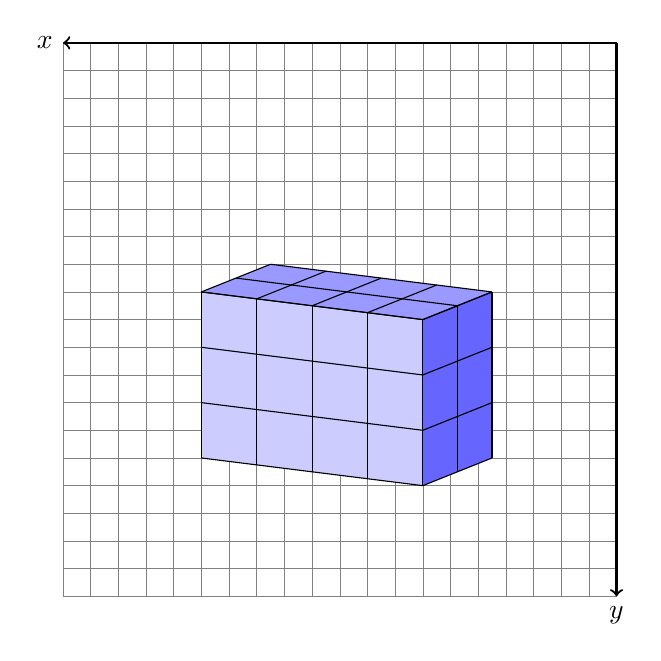
\begin{tikzpicture}
    \draw[help lines, step=1em] (0,0) grid (-20em, -20em);
    \draw[thick, ->] (0,0) -- (-20em, 0) node[left] {$x$};
    \draw[thick, ->] (0,0) -- (0, -20em) node[below] {$y$};
    
    \def\xsize{2};
    \def\ysize{3};
    \def\zsize{4};
  
    \begin{scope}[shift={(-15em, -15em)}, x={(2em,-0.25em)},y={(0em,2em)}, , z={(-1.25em,-0.5em)}]
      % Draw the front face
      \fill[blue!20] (0,0,0) -- (0,\ysize,0) -- (\zsize, \ysize,0) -- (\zsize,0,0) -- cycle;
      % Draw the top face
      \fill[blue!40] (0,\ysize,0) -- (0,\ysize,-\xsize) -- (\zsize, \ysize, -\xsize) -- (\zsize, \ysize,0) -- cycle;
      % Draw the right face
      \fill[blue!60] (\zsize,0,0) -- (\zsize,0,-\xsize) -- (\zsize, \ysize, -\xsize) -- (\zsize, \ysize,0) -- cycle;
  
      \foreach \x in {0,1, ..., \xsize}
      {
        \draw[black] (0, \ysize, -\x/\xsize * \xsize) -- (\zsize, \ysize, -\x/\xsize * \xsize);
        \draw[black] (\zsize,0,-\x/\xsize * \xsize) -- (\zsize, \ysize,-\x/\xsize * \xsize);
      }
  
      \foreach \y in {0, 1, ..., \ysize}
      {
        \draw[black] (0,\y/\ysize * \ysize,0) -- (\zsize,\y/\ysize * \ysize,0);
        \draw[black] (\zsize,\y/\ysize * \ysize,0) -- (\zsize,\y/\ysize * \ysize,-\xsize);
      }
  
      \foreach \z in {0, 1, ..., \zsize}
      {
        \draw[black] (\z/\zsize * \zsize,\ysize,0) -- (\z/\zsize * \zsize,\ysize,-\xsize);
        \draw[black] (\z/\zsize * \zsize,0,0) -- (\z/\zsize * \zsize,\ysize,0);
      }
    \end{scope}
  \end{tikzpicture}
  \caption{An example of MPI Cartesian topology Scheme of $24$ processors.}
  \label{FIG_MPI_TOPOLOGY_24_PROCS}
\end{figure}

\paragraph{Determine MPI datatypes for communication}
In order to do MPI communications, the source and the destination of every process are necessary, also the datatype.
When working with the meta-designed multidimensional matrix, we need to utilize the function \texttt{MPI\_Type\_Create\_subarray} to 
create essential halo datatypes.
\begin{algorithm}
  \begin{algorithmic}[1]
    \STATE \texttt{array\_size}, \texttt{array\_subsize}, \texttt{array\_starts=\{0\}} \hfill \#\texttt{std::array<Integer, NumD>}, the information of matrix.
    \FOR {i = 0 : NumD}
      \STATE Split tasks in dimension \texttt{i} by calling \texttt{decomposition}
      \STATE \texttt{array\_size = }local shape
      \STATE \texttt{array\_subsize = array\_size - 2}
    \ENDFOR
    \FOR {i=0 : NumD}
      \STATE \texttt{temp = array\_subsize[i]} \hfill \# Store the number temporally.
      \STATE \texttt{array\_subsize[i] = 1}
      \STATE \texttt{MPI\_Type\_Create\_subarray
      } and \texttt{MPI\_Type\_commit()} \hfill \# Create halo in dimension \texttt{i} and commit.
      \STATE Restore temporal array sub-size.
    \ENDFOR
  \end{algorithmic}
\end{algorithm}

\begin{figure}[htbp]
  \centering
  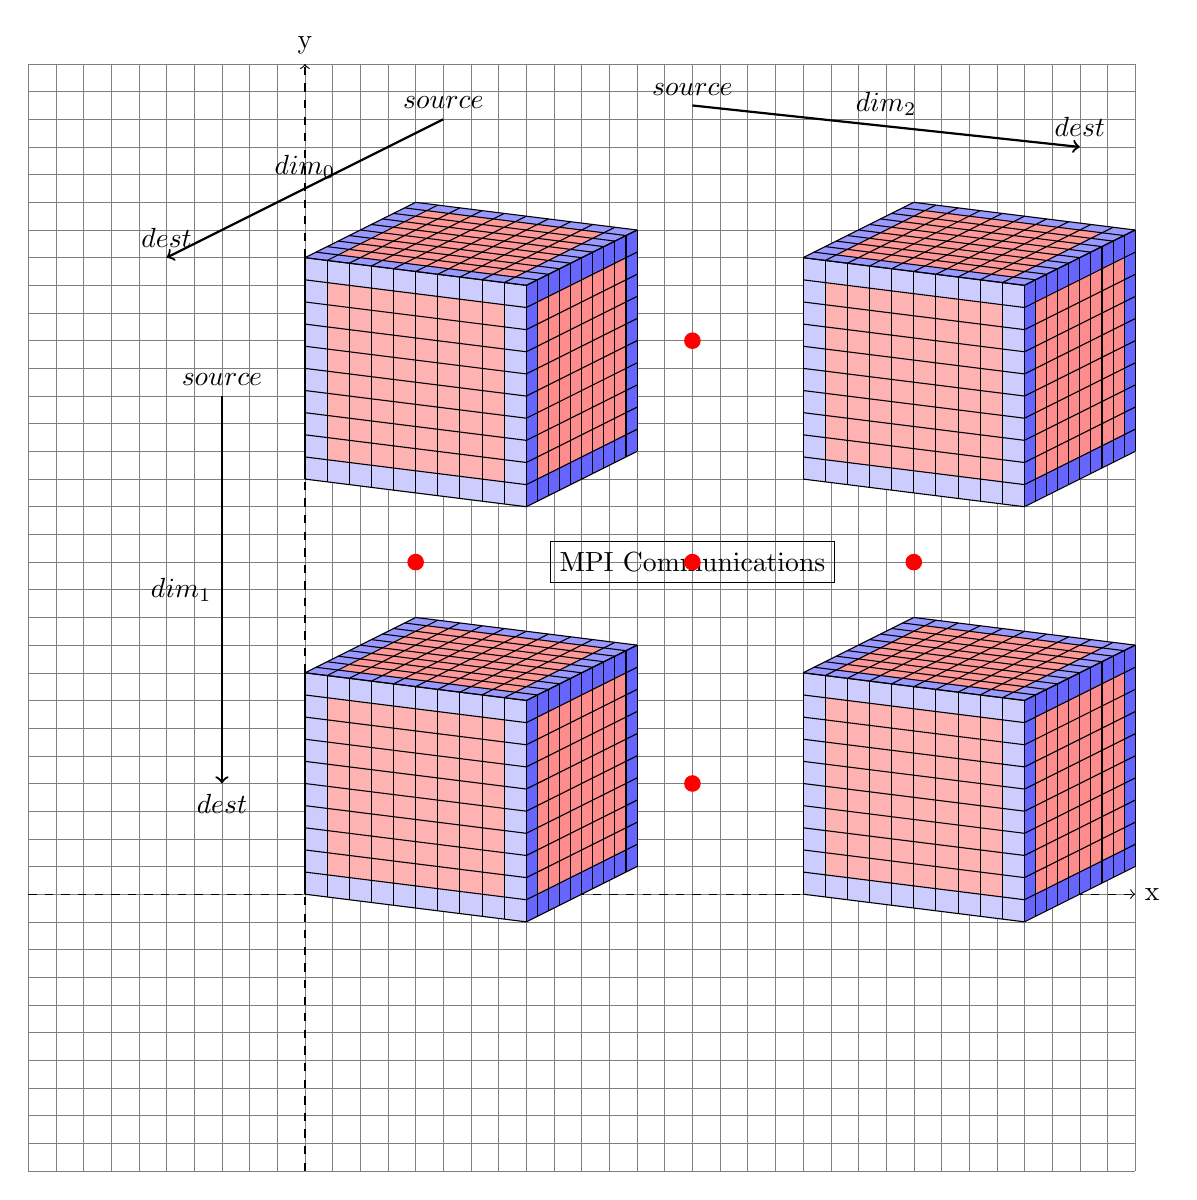
\begin{tikzpicture}
    % Draw a grid with steps of 1 cm
    \draw[help lines, step=1em] (-10em,-10em) grid (30em,30em);
  
    % Draw axes
    \draw[dashed,->] (-10em,0) -- (30em,0) node[right] {x};
    \draw[dashed,->] (0,-10em) -- (0,30em) node[above] {y};
  
    \draw[thick,->] (5em, 28em) -- (-5em, 23em) node[pos=0, above] {$source$} node[pos=0.5, above] {$dim_0$} node[pos=1, above] {$dest$};
    \draw[thick,->] (-3em, 18em) -- (-3em, 4em) node[pos=0, above] {$source$} node[pos=0.5, left] {$dim_1$} node[pos=1, below] {$dest$};
    \draw[thick,->] (14em, 28.5em) -- (28em, 27em) node[pos=0, above] {$source$} node[pos=0.5, above] {$dim_2$} node[pos=1, above] {$dest$};
  
      % Define a local macro to draw a cube at a given position
      \def\drawcube#1#2{
        \begin{scope}[shift={#1}, x={(0.8em,-0.1em)}, y={(0em,0.8em)}, z={(0.4em,0.20em)}]
          \def\size{#2}
          % Draw the front face
          \fill[blue!20] (0,0,0) -- (0,\size,0) -- (\size, \size,0) -- (\size,0,0) -- cycle;
          % Draw the top face
          \fill[blue!40] (0,\size,0) -- (0,\size,\size) -- (\size, \size, \size) -- (\size, \size,0) -- cycle;
          % Draw the right face
          \fill[blue!60] (\size,0,0) -- (\size,0,\size) -- (\size, \size, \size) -- (\size, \size,0) -- cycle;
  
          \fill[red!30] (1,1,0) -- (1,\size-1,0) -- (\size-1, \size-1,0) -- (\size-1,1,0) -- cycle;
          \fill[red!40] (1,\size,1) -- (1,\size,\size-1) -- (\size-1, \size, \size-1) -- (\size-1, \size,1) -- cycle;
          \fill[red!45] (\size,1,1) -- (\size,1,\size-1) -- (\size, \size-1, \size-1) -- (\size, \size-1,1) -- cycle;
  
          % Draw the grid
          \foreach \x in {0,1,...,\size} {
            \draw[black] (\x,0,0) -- (\x,\size,0);
            \draw[black] (0,\x,0) -- (\size,\x,0);

            \draw[black] (\size,\x,0) -- (\size,\x,\size);
            \draw[black] (\size,0,\x) -- (\size, \size,\x);

            \draw[black] (\x,\size,0) -- (\x,\size,\size);
            \draw[black] (0,\size,\x) -- (\size, \size,\x);
          }
        \end{scope}
      }
  
      % Draw the first cube at (0,0) with size 8
      \drawcube{(0em, 0em)}{10}
      \drawcube{(18em, 0em)}{10}
      \drawcube{(0em, 15em)}{10}
      \drawcube{(18em, 15em)}{10}
        
      \node[draw, minimum width = 3em, minimum height = 1.5em, align=center] at (14em,12em) {MPI Communications};
    
      \fill[red] (14em,12em) circle (3pt);
      \fill[red] (14em,4em) circle (3pt);
      \fill[red] (14em,20em) circle (3pt);

      \fill[red] (4em,12em) circle (3pt);
      \fill[red] (22em,12em) circle (3pt);
    \end{tikzpicture}  
  \caption{A 3D MPI Communication Scheme of $8$ processors between $3$ dimension matrices.}
  \label{FIG_MPI_3D_Example_SCHEME}
\end{figure}


\subsection{Template Distributed Multi-dimension Matrix Design}\label{SEC:SUB:Distributed_Matrix_Design}
\subsubsection{Detail Object Design}
Adhering to the STL safety routines, I chose to create detail template class object, hidden from users,
named \texttt{\_\_array\_Cart<class \_\_T, \_\_size\_type \_\_NumD>}.
Here, the \texttt{\_\_T} represents the value type, \texttt{\_\_size\_type} specifies the type of number of dimensions.
Since it is internal and not exposed from users, I decided to directly use other detail objects as member variables rather than 
smart pointers.
In this context, Cartesian matrix has public member variables \texttt{\_\_array} and \texttt{topology::Cartesian},
and provides memory operations. 
But the copy, move constructors and assignment operators are removed.
This approach enhances both performance both performance and simplicity by avoiding unnecessary abstractions in the internal design 
while maintain a robust memory management.

\paragraph{Distributed operator <<}
The STL os stream operator \texttt{<<} prints the matrices of all processes in sequence which build on multidimensional matrix's. 
Thus the Unix standard \texttt{fflush} function is utilized for flushing the cache in terminal, to ensure the stdout is print immediately.

\subsubsection{User Interface Design}
The \texttt{array\_Cart<class T, size\_type NumD>} is an object exposed to users, whereas only provides limited access to member variables by smart pointer.
As the size of matrices stored, it becomes clear that memory management is critically important. 
Secondly, especially in MPI distributed matrices, exposing direct memory access by set it to public member is dangerous. 
With the profits mentioned in Section \ref{SEC:RAII}, using unique pointer brings more benefits in this scenario, 
\begin{enumerate}
  \item MPI program memory management has higher complexity level. 
  Adhering RAII routines, the resources are bind with object, including MPI objects, and will be deleted as the object destructed. 
  \item Simplifying Concurrency Control. Synchronization between processes is a critical issue. 
  By using the RAII, user could unsure the resources are locked or released automatically, preventing the risk of deadlocks and resource contention.
\end{enumerate}



\subsection{Template Function Gather of Cartesian Distributed Multi-dimension Matrix}
The inverse of distributing multidimensional matrices 
[Sec. \ref{SEC:SUB:Distributed_Matrix_Design}]
based on MPI Topology 
[Sec. \ref{SEC:SUB:MPI_Topology}] 
is gather all distributed matrices to root from all processes.
Unlike operating on ordinary objects, gather function is operating on template objects which makes MPI operations harder.
Rather than applying full specialization for each dimension, continuing using meta-programming skills on this brings couple promotions
\begin{enumerate}
  \item Meta-programming, significantly reduce the redundancy of code, where I found the gathering operations on each dimension are highly repeatable. 
  \item Creating MPI Datatype also can be simplified due to the benefits of polymorphism. Especially when handling the high-dimension matrices.
  \item Using template makes the function is eligible to apply on various value basic data types, \texttt{Float}, \texttt{Double} etc, and provides consistency when handling uncompatible data type.
  \item Meta-polymorphism is more likely to have better performance, the initializations of template function are completed in compile time, which means there will be no run-time type-checking or type-casting.
\end{enumerate}


\subsubsection{Implement of Gather}
The \texttt{Gather} has following prototype, with the value type of entities of matrices and number of dimension as \texttt{size\_type},
\begin{lstlisting}[
  style=customCpp,
  caption={Prototypee of \texttt{final\_project::mpi::Gather}}]
  template <typename T, size_type NumD> 
  void Gather(gather, loc, root);
\end{lstlisting}
where:
\begin{itemize}
  \item \texttt{gather} is a reference of \texttt{multi\_array::array\_base<T, NumD>}, which will collect local data and store as the global matrices.
  \item \texttt{loc}    is a constant reference of the local matrices of \texttt{const array\_Cart<T, NumD>}, which holds local values and will sending data to root process.
  \item \texttt{root}   is a constant \texttt{Integer}, stands for the rank of root process.
\end{itemize}
The main idea of this function follows the following algorithm
\begin{algorithm}
  \caption{Scheme of Gather local matrices to Root process.}
  \begin{algorithmic}[1]
    \STATE Create gather object.
    \STATE Determine the sending address and sizes on each dimension, considering the boundary.
    \STATE Send the local size, starts information to root process.
    \IF{rank != root}
      \STATE Create local sub-array MPI Datatype, send to root.
    \ELSE  
      \FOR{pid = 0 : number process}
        \IF {pid != root}
          \STATE Root creates MPI Datatype using received local size information.
          \STATE Root receives data from others.
        \ELSE 
          \STATE Move the values by recursively applying local memory copy.
        \ENDIF
      \ENDFOR
    \ENDIF
  \end{algorithmic}
\end{algorithm}

\subsubsection{Determine Local Information}
Initially, the matrix object is designed on compatibility, it can read/load data from binary \texttt{.bin} files.
Thus the distributed matrices are saving  on the root process, by iterating through all processes, calculating the sizes 
and start indices on each dimension. Receiving them using \texttt{MPI\_Recv} from other processes send by \texttt{MPI\_Send}.

Considering boundaries, given a $D$ dimensional matrices, with global size $\mathcal{N}_{glob} = \{N_{glob}^d + 2\}_{d = 0}^{D-1}$.
The local matrices has shape $\mathcal{N}_{loc} = \{N_{loc}^d+2\}_{d=0}^{D-1}$, starts from $\mathcal{S} = \{s_d\}$ and ends from $\mathcal{E} = \{e_d\}$ globally.
In the $d$ dimension, as long as the matrix starts $s_d$ equals to $1$, it aligns the global boundary from source site which means the index should step back to $0$ to 
include the boundary. 
In other side, the global boundary locates at the contiguous address in $d$ dimension, 
the matrix should send a more dice in this dimension, which means the sending size $N_{loc}^{d} + 1$.
Moreover, for the special case when there is only one process. 

Adhering the RAII design, Gather function is exposed to user, thus I have not apply \texttt{swap} memory operation between Cartesian distributed matrices and none-distributed matrix just 
for handling the corner case. 
Eventually, I solve this by introducing an additional variable called \texttt{back}, which means the Root will copy for layer of data to another matrix. 
By default, \texttt{back} is $0$, and will be set to $1$ if and only if the number of process is $1$. 

With above analysis, the scheme of find local information follows 
\begin{algorithm}
  \caption{Scheme of Finding Local Sending Information: starts, shapes, indexes.}
  \label{ALG:SCHEME:Find_LOCAL_SEND_INFO}
  \begin{algorithmic}[1]
    \STATE Make copies of local shape \texttt{N\_cpy}, starts \texttt{starts\_cpy}.
    \STATE \texttt{back = 0}                           \hfill \# For handling $1$ process case.
    \IF{number process == 1}
      \STATE \texttt{++back}
    \ENDIF
    \STATE \texttt{index = \{1, 1, ..., 1\};}  \hfill \# Default sending index of local matrices.
    \FOR{d = 0 : NumD}
      \IF{starts[d] == 1}
        \STATE \texttt{-- starts\_cpy[d], --index[d]}
        \STATE \texttt{++ N\_cpy[d]}
      \ENDIF
      \IF{ends[d] == global\_shape[d] - 2}
        \STATE \texttt{++N\_cpy[d]}
      \ENDIF
      \STATE \texttt{MPI\_Gather( ..., Root)}  \hfill \# Send \texttt{starts\_cpy}, \texttt{N\_cpy} to Root;
    \ENDFOR
  \end{algorithmic}
\end{algorithm}

\subsubsection{Creating Send/Recv MPI Datatype}\label{SEC:Creating_Send/Recv_MPI_Datatype}
Local MPI communications are low efficient operations comparing to local memory copy operation, \texttt{memcpy} was used to 
recursively copy contiguous data from local matrix to global matrix exclusively on root process.
In a matrix with undefined dimension, creating data types for communicating is harder than in a specialized matrix.
For the none-root processes, they should send their data without ghost values, thus 
the \texttt{MPI\_Type\_create\_subarray} was used to create a sub-array \texttt{MPI\_Datatype} for sending message to root process.
\begin{lstlisting}[
  style=customCpp,
  caption={Routine for creating sub-array \texttt{MPI\_Datatype} as send buffer.}, 
  label={LST:mpi_subarray}]
  MPI_Type_create_subarray( 
      dimension,                     /// Dimension of this array  : NumD
      array_sizes.data(),            /// shape of local array     : local_shape
      array_subsizes.data(),         /// shape of sub-array       : N_cpy
      array_starts.data(),           /// starting coordinates     : {0, 0, ..., 0}
      MPI_ORDER_C,                   /// Array storage order flag : Row major in C/C++
      value_type,                    /// Old MPI Datatype         : get_mpi_type<T>()
      &sbuf_block);                  /// New MPI Datatype
\end{lstlisting}
The local arrays have shape $\mathcal{N}_{loc}$, and the sub-arrays have shape $\{N\_{cpy}\}_{d=0}^{D-1}$ determined by above routines 
                                            [Alg. \ref{ALG:SCHEME:Find_LOCAL_SEND_INFO}]
respectively, the starts indexes are unified as $0$s.
On the root process, the only difference is that the global shape of array \texttt{array\_sizes} are equal to the shape of global matrix.

\subsubsection{Local Copy Recursive Function}
The \texttt{memcpy} can only copy limited data to global matrix once,
since the elements we want to gather are not aligning on contiguous memory, 
but only a small amount of them - on the $0$ dimension - are continuously located.
Dut to the dimension of matrix is polymorphic and from the efficiency concern mentioned above 
            [Sec. \ref{SEC:Creating_Send/Recv_MPI_Datatype}],
the smallest copy operation using \texttt{memcpy} was encapsulated in a lambda function for recursively call and only visible in limited scope.

\begin{algorithm}
  \caption{\texttt{copy\_recursive(size\_type)}: Copy data using \texttt{memcpy} on given dimension}
  \label{}
  \begin{algorithmic}[1]
    \STATE Given current dimension \texttt{dim}.
    \IF{\texttt{dim == Num - 1}} 
      \STATE 
          \texttt{memcpy(}                                                    \hfill \# Copy data from local to global.\\
          \texttt{\: gather.begin() + gather.get\_flat\_index(loc\_idx),}     \hfill \# Get saving index in global matrix.\\
          \texttt{\: loc.data() + loc.get\_flat\_index(loc\_idx),}            \hfill \# Get copy start address of local matrix.\\
          \texttt{\: n\_list\_cpy[dim][pid] * sizeof(T) }                     \hfill \# Number of elements.\\
          \texttt{);}
    \ELSE 
      \FOR{\texttt{i = start\_cpy[dim] : loc.ends[dim] + back}}
        \STATE \texttt{local\_indexes[dim] = 1}     
        \STATE \texttt{copy\_recursive(dim + 1)}                    \hfill \# Recursive calling, copy next dimension.
      \ENDFOR
    \ENDIF
  \end{algorithmic}
\end{algorithm}

\subsubsection{Performace}
Gather function is a computationally expensive operation when the scale is large and runs across thousands of processes. 
With this reason, gathering results is not a optimal choice for getting results in practical.
However, the performance balancing is still important since helpful for debugging and stay a health routine of coding.
In a brief, I specific designed some performance tunning features for following reasons
\begin{enumerate}
  \item Using lambda function can slow down the performance, however, gather operation is not always the core of a program since it's an IO operation for debugging or 
  get the final results at the very end. 
  Besides, it's only available when the root process is receiving data, which is a small scope compare to the other parts.
  In all the drawback can be ignored in this case.
  \item The gather matrix is only initialized when we need gather the results.
  The reason for initializing gather object in this function, is that gather matrix is conventionally very large. 
  If it is create in advance, it will consuming large amount of memory space, which will reduce the rate of memory hit rate, 
  affect the speed of latter computing.
  \item Adhering RAII routine, I chose to make an copy of each parameters of local and global metrics. 
  While these objects are relatively short, creating them locally could help us make the original data safe, and make them have higher chance stored in register or cache 
  which a lot faster than reading/writing from/to memory.
\end{enumerate}

\subsection{Parallel MPI-IO for Distributed Matrices}
Building a gather function is convenient indeed, it allows us collecting data from all other processors.


% \subsubsection{Pure Message Passing Parallel}
% \subsubsection{Hybrid Parallel}

\subsection{Physics Informed Neural Networks}
\subsubsection{CUDA parallel}
\subsubsection{Hybrid Parallel}